\documentclass[11pt,a4paper]{article}

% For å kunne skrive norske tegn.
\usepackage[utf8]{inputenc}

% For å inkludere figurer.
\usepackage{graphicx}

% Ekstra matematikkfunksjoner.
\usepackage{amsmath,amssymb}

\usepackage[section]{placeins}

\usepackage{hyperref}
\hypersetup{%
  colorlinks=true, % hyperlinks will be black
  urlcolor=red,
  linkcolor=red
}

\usepackage{fancyvrb}

\newenvironment{code}
  {
    \VerbatimEnvironment
    \vskip\baselineskip\hrule
    \begin{Verbatim}[xleftmargin=7pt]%
  }
  {\end{Verbatim}\hrule\vskip\baselineskip}

% Må inkluderes for blant annet å få tilgang til kommandoen \SI (korrekte måltall med enheter)
\usepackage{siunitx}

  % Prikk som multiplikasjonstegn (i steden for kryss).
  \sisetup{exponent-product = \cdot}

  % Pluss-minus-form på usikkerhet (i steden for parentes).
  \sisetup{separate-uncertainty = true}

% For å få tilgang til finere linjer (til bruk i tabeller og slikt).
\usepackage{booktabs}

% For justering av figurtekst og tabelltekst.
\usepackage[font=small,labelfont=bf]{caption}

% Subsections A, B,
\renewcommand{\thesubsection}{\Alph{subsection}}

% Disse kommandoene kan gjøre det enklere for LaTeX å plassere figurer og tabeller der du ønsker.
\setcounter{totalnumber}{5}
\renewcommand{\bottomfraction}{0.95}
\renewcommand{\floatpagefraction}{0.35}

\begin{document}

  % Rapportens tittel:
  \title{Lab 5: Information Access \\ \large{TDT4275: Natural Language Interfaces}}
  \author{Jonas Myrlund}

  % Her ber vi LaTeX om å lage tittelen (til nå har vi bare sagt hva den skal inneholde):
  \maketitle

  \section{Written Assignments} % (fold)
  \label{sec:written_assignments}

    \subsection{Using either web searches or a large corpus, devise a query using a polysemous word.} % (fold)
    \label{sub:using_either_web_searches_or_a_large_corpus_devise_a_query_using_a_polysemous_word_}

      I want to find out more about large cranes -- the bird. I start out with the following query:
      ``large crane''.

      See figure \ref{fig:large_crane_google} for the initial results using Google\footnote{\url{https://google.com/search?q=large+crane}}.

      \begin{figure}
        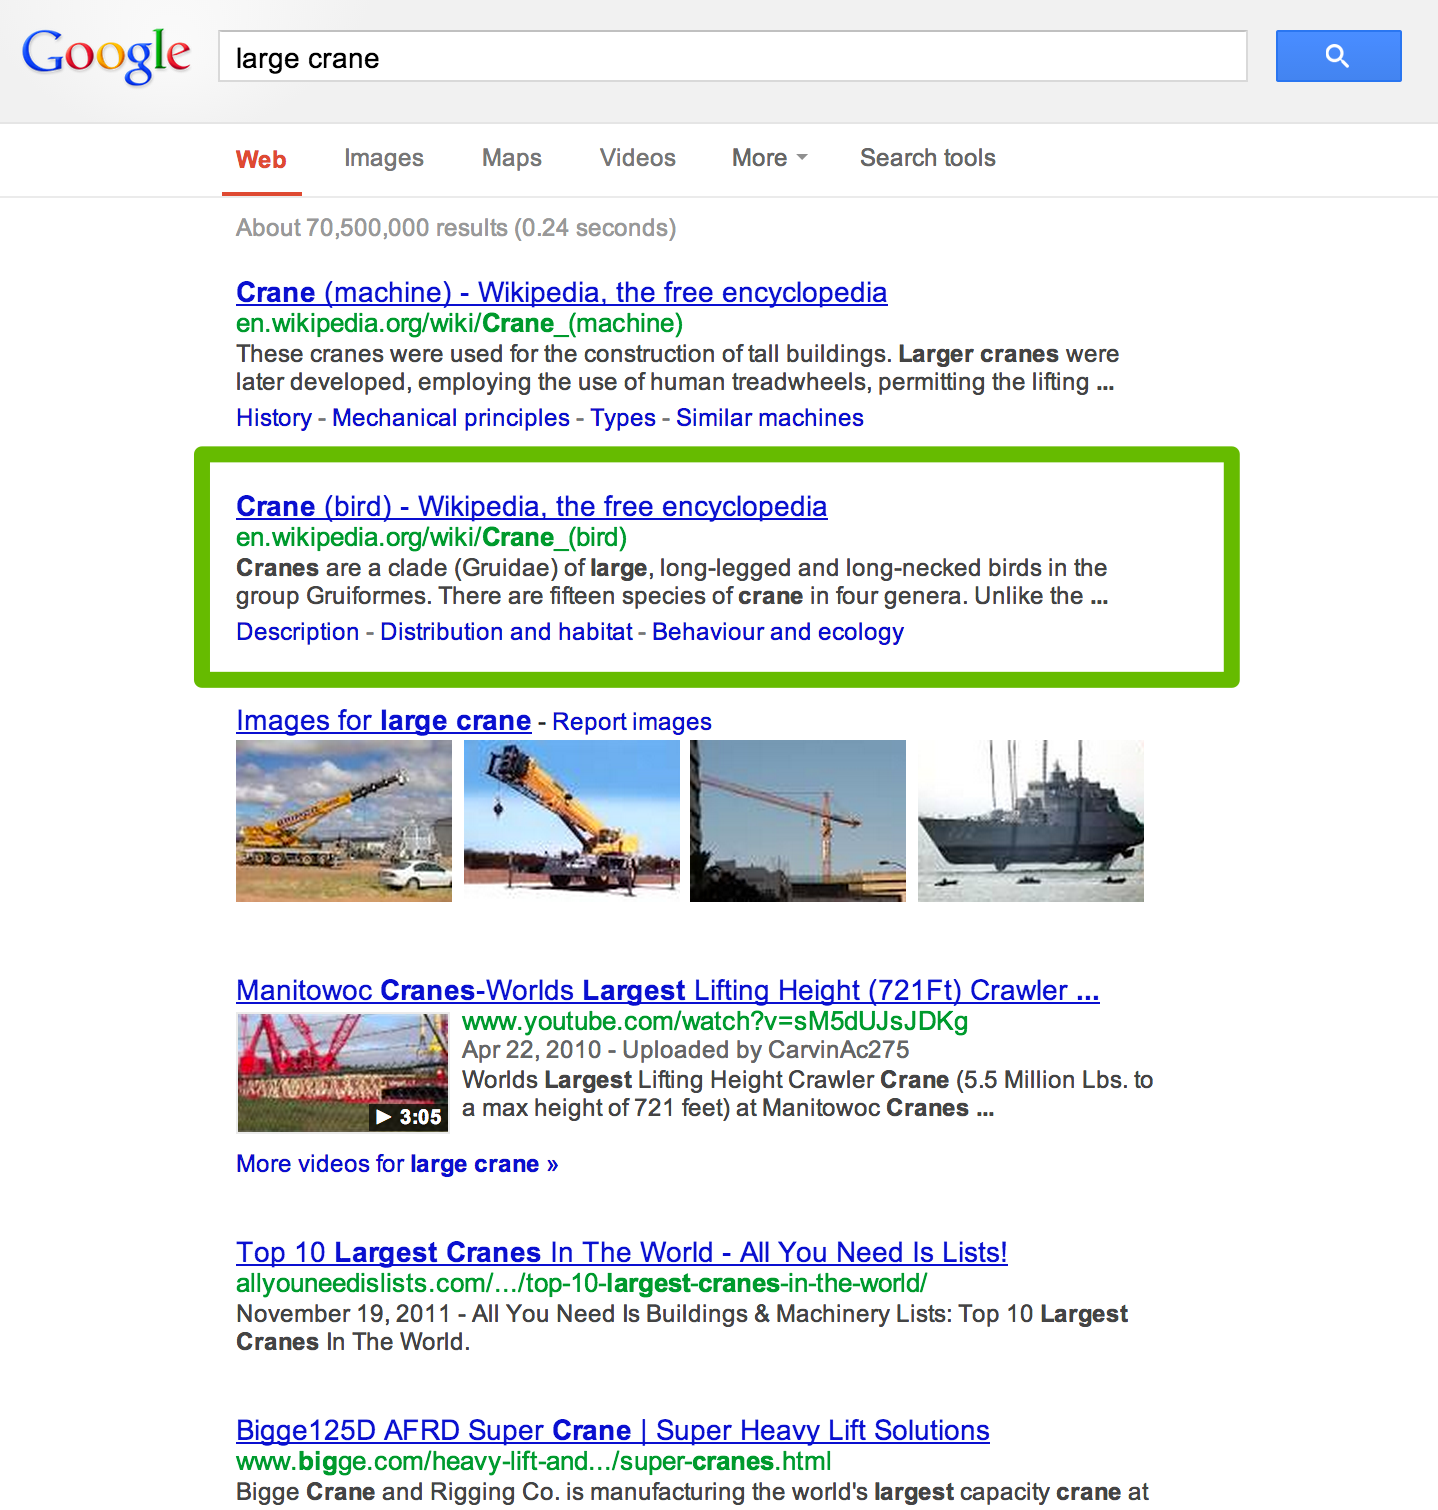
\includegraphics[width=0.95\textwidth]{imgs/large_crane_google}
        \caption{Google yields only one relevant search result when searching for ``large crane''.}
        \label{fig:large_crane_google}
      \end{figure}

    % subsection using_either_web_searches_or_a_large_corpus_devise_a_query_using_a_polysemous_word_ (end)

    \subsection{Then, devise two or three alternate queries which help to disambiguate the polysemous word and repeat the search.} % (fold)
    \label{sub:then_devise_two_or_three_alternate_queries_which_help_to_disambiguate_the_polysemous_word_and_repeat_the_search_}

      The query ``large crane'' could be less ambiguous in the following ways:

      \begin{enumerate}
        \item ``large crane bird''
        \item ``large crane feathers''
      \end{enumerate}

      As figure \ref{fig:large_crane_bird_google} exemplifies, these queries result in only documents relating to the \emph{bird sense} of the word \emph{crane}.

      \begin{figure}
        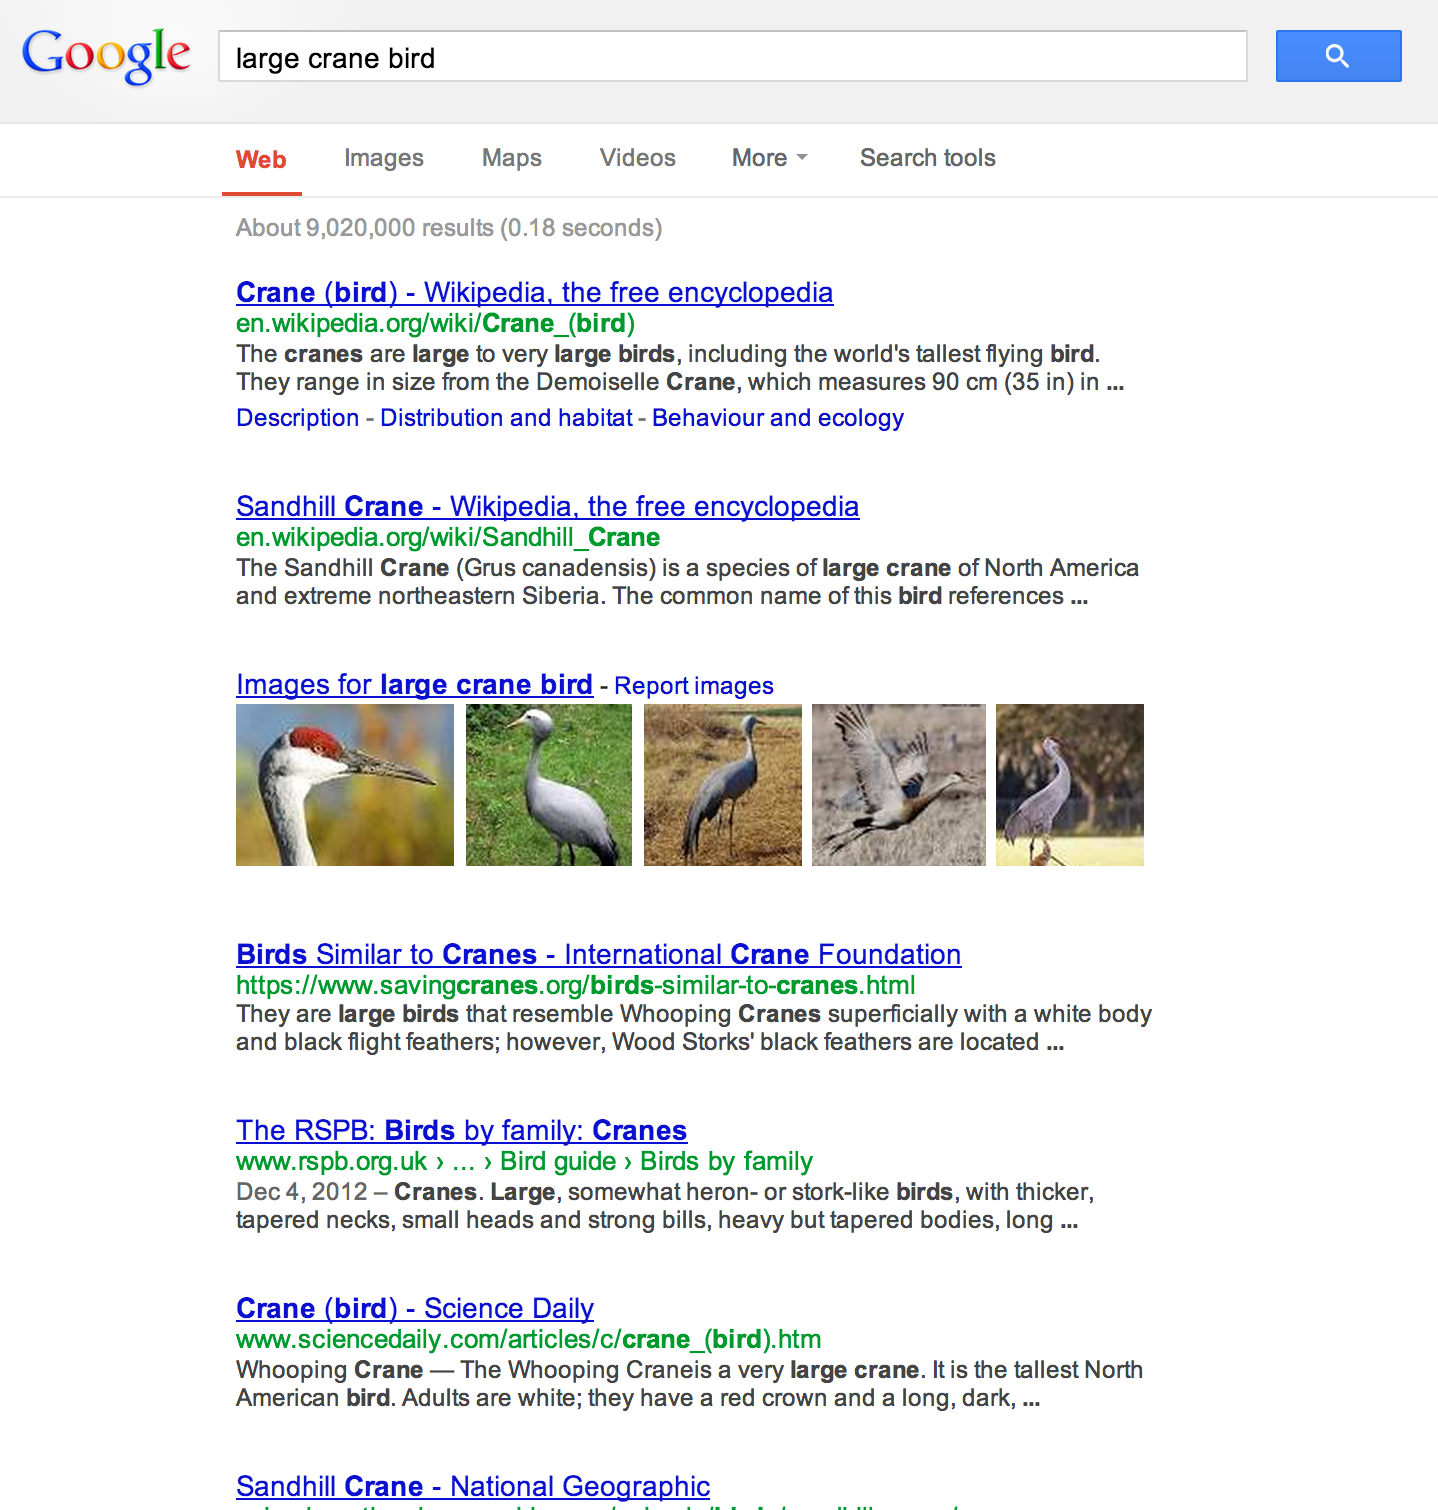
\includegraphics[width=0.95\textwidth]{imgs/large_crane_bird_google}
        \caption{When adding the term ``bird'' to the query, all the top results are relevant.}
        \label{fig:large_crane_bird_google}
      \end{figure}

    % subsection then_devise_two_or_three_alternate_queries_which_help_to_disambiguate_the_polysemous_word_and_repeat_the_search_ (end)

    \subsection{For each query, classify each of the top 10 search results as correct or incorrect.} % (fold)
    \label{sub:for_each_query_classify_each_of_the_top_10_search_results_as_correct_or_incorrect_}

      Again, I will be using Google for the queries.

      \subsubsection{Query: ``large crane''} % (fold)
      \label{ssub:query_large_crane_}

        The query yields only one correct document: the second search result.
        The others documents relate to the wrong sense of the word.
        For details, see figure \ref{fig:large_crane_google}.

      % subsubsection query_large_crane_ (end)

      \subsubsection{Queries: ``large crane bird'' and ``large crane feathers''} % (fold)
      \label{ssub:query_large_crane_bird_}

        For both these queries, all the first 10 search results relate to the right sense of the polysemous word in Google.

        Yahoo! and Bing, however, both give three documents relating only to feathers, which is not what is wanted.

      % subsubsection query_large_crane_bird_ (end)

    % subsection for_each_query_classify_each_of_the_top_10_search_results_as_correct_or_incorrect_ (end)

    \subsection{Create an interpolated precision-recall curve comparing the accuracy of each of the queries.} % (fold)
    \label{sub:create_an_interpolated_precision_recall_curve_comparing_the_accuracy_of_each_of_the_queries_}

      The recall values for the first query, ``large crane'', stagnates in that it gives only one correct document.
      Thus, the scales of the precision-recall curves do not overlap to a degree that makes it viable to plot them together.

      However, the curves quite clearly show the improvement adding a disambiguating term yields, when the precision axis is normalized to one. See figure \ref{fig:pr1}, \ref{fig:pr2} and \ref{fig:pr3}.

      \begin{figure}[h]
        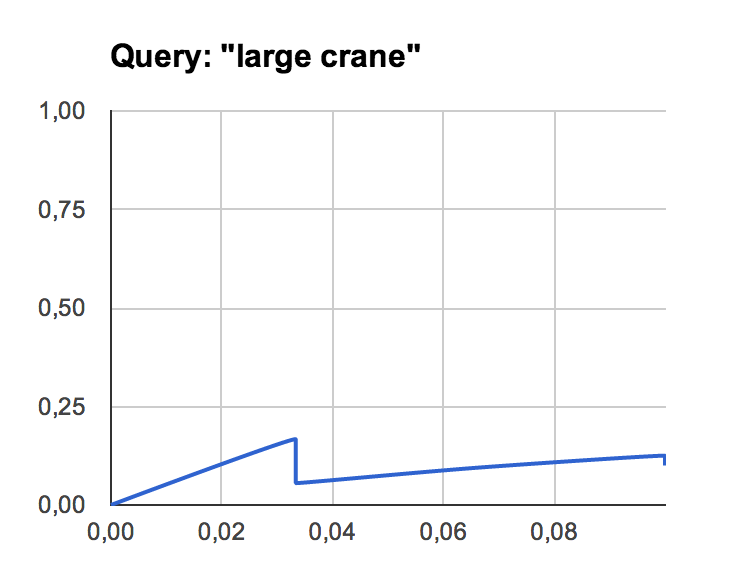
\includegraphics[width=0.85\textwidth]{imgs/large_crane_pr}
        \caption{Precision-recall curve for ``large crane''.}
        \label{fig:pr1}
      \end{figure}

      \begin{figure}[h]
        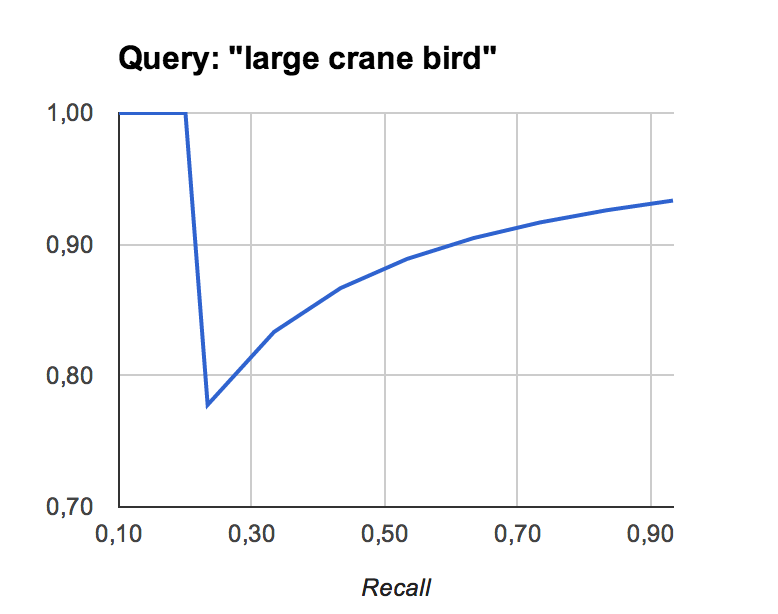
\includegraphics[width=0.85\textwidth]{imgs/large_crane_bird_pr}
        \caption{Precision-recall curve for ``large crane bird''.}
        \label{fig:pr2}
      \end{figure}

      \begin{figure}[h]
        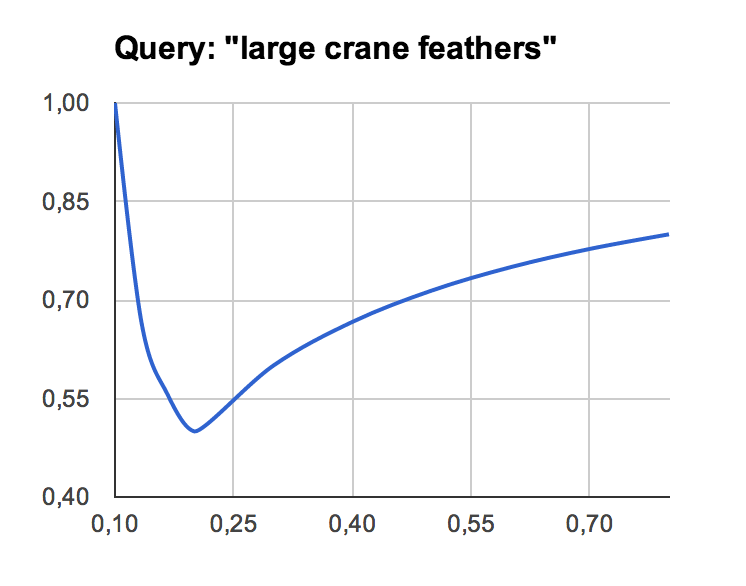
\includegraphics[width=0.85\textwidth]{imgs/large_crane_feathers_pr}
        \caption{Precision-recall curve for ``large crane feathers''.}
        \label{fig:pr3}
      \end{figure}

    % subsection create_an_interpolated_precision_recall_curve_comparing_the_accuracy_of_each_of_the_queries_ (end)

  % section written_assignments (end)

  \section{Information Retrieval} % (fold)
  \label{sec:information_retrieval}

    I went for a corpus traversed with Lynx from \url{http://www.sciencenews.org/}.

    \subsection{The effects of the various steps described in the assignment.}

      \paragraph{Turn the corpus into text form.}

      This really has no significant effect, as the corpus garnered from Lynx is already stripped of all HTML tags.

      \paragraph{Turn the file into a list of words.}

      Removes special characters, lowercases, and generally simplifies words into tokens, like this:
      \\

      \begin{tabular}{ll}
         \textbf{Before} & Animals' cognitive shortcomings are as revealing as their genius. \\
         \textbf{After}  & animals cognitive shortcomings are as revealing as their genius \\
      \end{tabular}
      \\

      \paragraph{Build word frequency tables.}

      This results in a series of \emph{term frequency} files, of the following format:

      \begin{code}
        0.00342987804878049        animals
        0.00114503816793893        cognitive
        0.00114503816793893        shortcomings
      \end{code}

      The number to the left denotes the term frequency of the word to the right.

      \paragraph{Create your own stop list.}

      This step is simply a matter of looking manually at some of the generated files and seeing which words are present in every document.
      These are manually extracted into a stop list.

      The beginning of my stop list looks like the following:

      \begin{code}
        a
        all
        the
        of
        and
        in
        for
        on
        or
      \end{code}

      \paragraph{Determine the terms' descriminative values.}

      This step calculates the IDF -- the inverse document frequency -- of each word found in the tokenized document collection.
      The IDF routine simply outputs each word together with the inverse of the term frequency over the entire corpus.

      \paragraph{Experiment with a simple search engine.}

      Searching for ``physical society'' should probably lead to a document summarizing a recent meeting in the Physical Society.

      Running \texttt{echo physical society | ../bin/search.perl -i idflist -e tfs} results in the following
      (please note that the numbers to the left are a result of some heavy playing around with weighting TF and IDF terms):

      \begin{code}
        2430.451300474519204 lnk00000036.tfs
        0.451300474519204 lnk00000037.tfs
        0.204453275655133 lnk00000030.tfs
      \end{code}

      As expected, the raw document \texttt{lnk00000036.txt} is the document we were looking for.

      Using a stoplist has no significant effect with the configuration used in the example above.

  % section information_retrieval (end)

  \section{Text Summarisation} % (fold)
  \label{sec:text_summarisation}

    \subsection{} % (fold)

      The SweSum summariser\footnote{\url{http://swesum.nada.kth.se/index-eng-adv.html}} is first and foremost a single DOC summariser.
      Furthermore, it accepts keywords to aid in the summarisation, in this way handling a sort of QUERY input as well.

      The summariser is an EXTRACT summariser -- it selects what it deems the most relevant sentences, and concatenates them together.

    % subsection  (end)

    \subsection{} % (fold)

      The first article I've chosen to summarise is one about seafowl being killed by seismic shooting under water\footnote{\url{http://www.nrk.no/nyheter/distrikt/troms_og_finnmark/1.10996526}}.
      The summaries are attached in appendix \ref{sub:article_1}.

      The second article is a short sports article\footnote{\url{http://www.nrk.no/sport/fotball/tyson-stotter-suarez-1.10997215 }}. The summaries are attached in appendix \ref{sub:article_2}.

    % subsection  (end)

    \subsection{} % (fold)

      I would rank the summaries in the following way:

      \begin{enumerate}
        \item 25\% version of article \ref{sub:article_2}.
        \item 50\% version of article \ref{sub:article_1}.
        \item 50\% version of article \ref{sub:article_2}.
        \item 25\% version of article \ref{sub:article_1}.
      \end{enumerate}

      \paragraph{My favorite summary} is extremely short.
      However, it highlights the important parts of the article, while leaving out a lot of the quite uninteresting parts.

      The real story -- the message -- is in the first couple of paragraphs, whereas the latter half of the article raves about how the two people involved heard about each other and started following each other on Twitter -- very peripheral material.
      This last bit is all left out in the summary, and would probably never be missed by anyone.

      \paragraph{The worst summary in my opinion} fails to acknowledge the different opinions within the original article.
      The article is split in two, the first half presenting one view, the other half presenting an opposing view, and it does not conclude one way or another.
      The summary, however, presents only the first view, and fails to even mention the controversy highlighted by the latter half of the article.

      \paragraph{I can think of two ways of making sure the omitted sentences are included:}
      to \emph{identify the headlines} and include at least one central sentence from each of these headlined sections,
      and \emph{classifying the names of people involved}, ensuring that one quote from each interviewee is included in the summary.

    % subsection  (end)

  % section text_summarisation (end)

\appendix

\renewcommand{\thesubsection}{\thesection-\arabic{subsection}}

\section{Text summaries} % (fold)
\label{sec:text_summaries}

  \subsection{Article 1 -- ``Mener lundefuglene kan ha dødd på grunn av seismikkskyting''} % (fold)
  \label{sub:article_1}

    The original article can be found \href{http://www.nrk.no/nyheter/distrikt/troms_og_finnmark/1.10996526}{on NRK.no}.

    The \emph{25\% summary}:

    \begin{quotation}
      I forrige uke fant barnehageunger på tur i Botnfjæra i Dyfjord i Finnmark 11 døde lundefugler.
      Fisker og sekretær i Andøy Fiskarlag, Bjørnar Nicolaysen, mener konsekvensene av seismikkskytingene i Vesterålen, Lofoten og Senja er mye verre enn antatt.

      De døde lundefuglene som nylig ble funnet i fjæra i Dyfjord i Lebesby kommune i Finnmark kan skyldes trykkbølgene fra seismikkskyting, frykter Nicolaysen.

      – Lundefugl som annen sjøfugl er avhengig av maten som finnes under havflaten.

      Seismikkskyting er oljeindustriens viktigste redskap for å kartlegge mulige forekomster av olje og gass mange tusen meter under jordoverflaten, og er derfor definert som petroleumsvirksomhet i petroleumsloven. Det er blitt undersøkt konsekvensene av effektene av seismikk på havet.
    \end{quotation}

    The \emph{50\% summary}:

    \begin{quotation}
      I forrige uke fant barnehageunger på tur i Botnfjæra i Dyfjord i Finnmark 11 døde lundefugler.
      Fisker og sekretær i Andøy Fiskarlag, Bjørnar Nicolaysen, mener konsekvensene av seismikkskytingene i Vesterålen, Lofoten og Senja er mye verre enn antatt.

      De døde lundefuglene som nylig ble funnet i fjæra i Dyfjord i Lebesby kommune i Finnmark kan skyldes trykkbølgene fra seismikkskyting, frykter Nicolaysen.

      – Lundefugl som annen sjøfugl er avhengig av maten som finnes under havflaten. Dukker den ned der det skytes seismikk, så er den ferdig.

      Fisker Bjørnar Nicolaisen fra Andøy mener lundefuglene kan ha dødd på grunn av seismikkskyting.

      Seismikkskyting er oljeindustriens viktigste redskap for å kartlegge mulige forekomster av olje og gass mange tusen meter under jordoverflaten, og er derfor definert som petroleumsvirksomhet i petroleumsloven.

      – Det er ingen av oss som kjenner til episoder hvor seismikk har drept sjøfugl. Tvert om antar vi at sjøfugl svømmer under båten når den nærmere seg, og blir ikke påvirket i det hele tatt.

      – Jeg tviler på at lundefuglepisoden har noe med seismikk å gjøre.

      – Kan omfattende seismikkskyting påvirke fuglelivet? Det er blitt undersøkt konsekvensene av effektene av seismikk på havet. Det ble også gjort undersøkelser på sjøpattedyr.

      De har også deltat i overvåkings- og kartleggingsprogram for norske sjøfugler (Seapop), hvor seismikk og sjøfugl aldri tidligere har vært et tema.
    \end{quotation}

  % subsection article_1 (end)

  \subsection{Article 2 -- ``Bite-Tyson tar bite-Suarez i forsvar''} % (fold)
  \label{sub:article_2}

    The original article can be found \href{http://www.nrk.no/sport/fotball/tyson-stotter-suarez-1.10997215}{on NRK.no}.

    The \emph{25\% summary}:

    \begin{quotation}
      Bite-Tyson tar bite-Suarez i forsvar
      – Han bet noen, sånt skjer, sier Mike Tyson.

      Etter Luis Suarez' siste skandale, søndagens biting av Chelsea-spiller Branislav Ivanovic, får han støtte fra noen som virkelig kan sette seg inn i situasjonen hans - bokselegenden Mike Tyson.

      Mange husker nok da Tyson satte tennene i Evander Holyfields øre under en boksekamp i 1997.
    \end{quotation}

    The \emph{50\% summary}:

    \begin{quotation}
      Bite-Tyson tar bite-Suarez i forsvar
      – Han bet noen, sånt skjer, sier Mike Tyson.

      Mike Tyson uttalte seg om Luis Suarez i et radioshow tirsdag.

      Etter Luis Suarez' siste skandale, søndagens biting av Chelsea-spiller Branislav Ivanovic, får han støtte fra noen som virkelig kan sette seg inn i situasjonen hans - bokselegenden Mike Tyson. De er og var begge i verdenstoppen i sine idretter, og begge har brukt biting i forsøk på å stanse sine motstandere.

      Mange husker nok da Tyson satte tennene i Evander Holyfields øre under en boksekamp i 1997.

      Følger Suarez på Twitter

      Etter biteepisoden søndag var det flere som merket seg at plutselig hadde bokselegenden begynt å ``følge'' Suarez på nettstedet Twitter.

      Tyson bekrefter at det var bitingen som gjorde ham oppmerksom på Liverpool-spilleren. Han kan vente seg flere kampers karantene.
    \end{quotation}

  % subsection article_2 (end)

% section text_summaries (end)

\end{document}















